\documentclass[conference,letterpaper]{IEEEtran}
\usepackage[T1]{fontenc}
\usepackage{mathptmx}
\usepackage{cite}
\usepackage{amsmath,amssymb}
\usepackage{graphicx}
\usepackage{array,booktabs}
\usepackage{balance}
\usepackage[colorlinks=true,linkcolor=blue,citecolor=blue,urlcolor=blue]{hyperref}
\urlstyle{same}
\setlength{\tabcolsep}{3pt}
\newcommand{\code}[1]{\texttt{#1}}
\begin{document}
\title{IsoLab: Executable Container Defenses and Multi-Tenant Reliability Evaluation}
\author{
\IEEEauthorblockN{Atharva Agrawal}
\IEEEauthorblockA{\textit{Indian Institute of Information Technology Dharwad}\\
Dharwad, India\\
23bds010@iiitdwd.ac.in}
\and
\IEEEauthorblockN{Niti Priya}
\IEEEauthorblockA{\textit{Indian Institute of Information Technology Dharwad}\\
Dharwad, India\\
23bcs087@iiitdwd.ac.in}
}
\hypersetup{pdftitle={IsoLab: Executable Container Defenses and Multi-Tenant Reliability Evaluation},
pdfauthor={Atharva Agrawal and Niti Priya},pdfsubject={Cloud SRE and Security}}
\maketitle

\begin{abstract}
Multi-tenant containers combine shared-resource interference with security exposure. IsoLab connects selected defenses from a 2025 container-security survey to executable checks and startup integrity enforcement, alongside provider-side interference observation motivated by a 2024 multi-tenant monitoring study. It integrates thirty configuration checks, resource controls, event detection, and a metadata canary. Historical three-tenant measurements show that hardening reduces median noisy-arm 99th-percentile latency from 16.463 to 5.617 milliseconds, a 65.9 percent reduction; both profiles meet the 25-millisecond target. Twelve tested exposure paths close while three positive controls remain functional. Eight expected insecure and seven expected hardened detections meet timing and attribution criteria. New experiments detect all ten independently injected snapshot configuration faults and correctly accept or reject all five isolated startup-integrity challenges. The contribution is an executable defense-to-evidence mapping with complementary reliability evaluation, rather than a new isolation primitive or a reproduction of the 2024 neural-network classifier. Results support feasibility within the measured scope; they do not establish comprehensive exploit resistance or superiority over either source work.
\end{abstract}

\begin{IEEEkeywords}
cloud security, site reliability engineering, multi-tenancy, container isolation, noisy neighbor
\end{IEEEkeywords}

\section{Introduction}
Cloud tenants depend on boundaries that preserve confidentiality and predictable resource access. A workload can suffer latency inflation when another tenant exhausts shared processor capacity, even without a direct compromise. Conversely, healthy request latency does not establish that networks, storage, or management interfaces are isolated. Assessing a cloud security mechanism therefore requires complementary evidence about resource interference, boundary enforcement, and detection.

Two recent studies motivate this work. \href{https://doi.org/10.1016/j.jnca.2024.103839}{Horchulhack \emph{et al.}}~\cite{qos2024} investigate provider-side detection of container interference using resource observations and learned temporal classification. \href{https://doi.org/10.1145/3715001}{Jarkas \emph{et al.}}~\cite{acm2025} organize container exploits and defenses into a security taxonomy. These studies motivate a practical question: how can selected defensive recommendations be connected to reproducible enforcement and reliability evidence in an accessible laboratory? IsoLab answers with a scoped implementation and explicit evidence boundaries. Its original R1--R4 requirement labels and five-axis check grouping retain their historical provenance in \href{https://doi.org/10.1186/2192-113X-1-11}{Gonzalez \emph{et al.}}~\cite{gonzalez}; they are not attributed to the recent papers.

IsoLab connects security controls to site reliability engineering (SRE) through a measurable latency objective and tenant-level resource observations. The study addresses four research questions:
\begin{itemize}
\item \textbf{RQ1:} Does the hardened configuration reduce processor interference relative to an intentionally insecure baseline?
\item \textbf{RQ2:} Are the tested tenant boundaries closed while required application and monitoring connectivity remains functional?
\item \textbf{RQ3:} Are benign isolation-breaking triggers detected within specified latency limits and with the expected workload attribution?
\item \textbf{RQ4:} Do selected defense checks and startup integrity enforcement reject their specified configuration and file-integrity faults?
\end{itemize}

Our contributions are: (1) a machine-readable crosswalk connecting selected 2025 survey defense themes to existing configuration checks and complementary observations; (2) startup hashing and executable/entry-script allowlisting, implementing a selected aspect of mitigation M2; (3) independent configuration-fault and integrity challenges, alongside historical latency, segmentation, and detection evidence; and (4) fail-closed evidence predicates and an interactive research interface. The system integrates established controls rather than introducing a new isolation primitive. Historical live runs and newly executed local challenges are reported separately.

\section{Background and Related Work}
\subsection{Recent Multi-Tenant Monitoring and Container Security}
Horchulhack \emph{et al.}~\cite{qos2024} combine engine and process-namespace observations with feature reduction and time-series classification, evaluated on a distributed containerized Big Data platform. IsoLab shares the provider-observation motivation but uses explicit CPU-sharing rules, PSI, resource controls, and a synthetic request-latency experiment. It does not reproduce the autoencoder, recurrent neural network, or four-host Kubernetes/Spark evaluation. Detector accuracy numbers from that study are therefore not directly comparable with IsoLab's deterministic trigger counts.

The 2025 ACM survey~\cite{acm2025} supplies an exploit/defense taxonomy rather than one reference algorithm. We implement selected software defenses and operationalize their validation. This complements the survey with executable local evidence; it neither replaces its breadth nor validates every associated vulnerability. Binary integrity checking, in particular, is scoped to startup under a trusted build and manifest.


Table~\ref{tab:positioning} distinguishes the source works from the present study by method and evidence. It establishes scope rather than a ranking: workloads, deployment sizes, and evaluation units differ.

\begin{table}[t]
\caption{Positioning Relative to the Two Main Source Works}
\label{tab:positioning}
\centering
\footnotesize
\renewcommand{\arraystretch}{1.13}
\begin{tabular}{@{}>{\raggedright\arraybackslash}p{.22\columnwidth}>{\raggedright\arraybackslash}p{.34\columnwidth}>{\raggedright\arraybackslash}p{.38\columnwidth}@{}}
\toprule
Work & Main method & Evidence and relationship \\ \midrule
Horchulhack et al. (2024)~\cite{qos2024} & Resource observation, feature reduction, temporal classification & Distributed-service interference detection; motivates our deterministic monitoring adaptation \\
Jarkas et al. (2025)~\cite{acm2025} & Exploit and defense taxonomy & Survey synthesis; supplies selected defensive recommendations \\
IsoLab & Configuration checks, resource controls, event rules, startup hashing & Local E1--E3 comparison plus E4--E5 challenges; no classifier superiority claim \\
\bottomrule
\end{tabular}
\end{table}

\subsection{Container Threats and Empirical Security Evaluation}
\href{https://doi.org/10.1109/ACCESS.2019.2911732}{Sultan \emph{et al.}}~\cite{sultan} distinguish security relationships within containers, between containers, and between containers and the host. This motivates making the trusted provider and host boundary explicit. \href{https://doi.org/10.1145/3274694.3274720}{Lin \emph{et al.}}~\cite{lin2018} evaluate Linux-container protection using real exploit cases and examine interacting kernel defenses. Their exploit-based evidence addresses a stronger attack mechanism than our benign probes and configuration mutations. IsoLab's closed endpoints and startup decisions consequently cannot be interpreted as equivalent exploit-resistance evidence.

\subsection{Virtualization Security Requirements}
The source survey~\cite{gonzalez} treats virtualization as an architectural security concern and emphasizes isolation and cross-VM attacks. IsoLab implements the engineering implications of its future-work requirements. It does not implement every branch of the taxonomy or claim that the historical literature deficit persists. Its check-coverage percentages quantify configuration posture and cannot be compared numerically with the survey's citation shares.

\subsection{Containers and Resource Observation}
NIST SP 800-190 describes containers as operating-system virtualization and discusses their security risks~\cite{nist}. Containers share a kernel, whereas hardware virtual machines use a different isolation boundary. This work is consequently a container adaptation of VM-oriented requirements, rather than a reproduction of a KVM, Xen, or VMware deployment.

\href{https://doi.org/10.1109/ISPASS.2015.7095802}{Felter \emph{et al.}}~\cite{felter} compare virtual-machine and Linux-container performance across workloads. This motivates distinguishing virtualization overhead from the interference question examined here. IsoLab compares two container configurations and does not measure a container-versus-VM performance advantage.

Linux cgroup v2 provides hierarchical resource control~\cite{cgroup}, while Pressure Stall Information (PSI) measures time lost to resource pressure~\cite{psi}. IsoLab combines these interfaces with configuration snapshots and engine events. Its explicit service-level objective (SLO) follows the SRE practice of assessing reliability through measurable service indicators~\cite{sre}. Here, the SLO is an experimental latency criterion at a fixed offered load, not a contractual availability guarantee.

\href{https://research.google/pubs/the-tail-at-scale/}{Dean and Barroso}~\cite{tail} explain why high-percentile latency matters in large services. IsoLab uses p99 as a tenant-visible indicator, while recognizing that its synthetic single-service workload does not reproduce the fan-out behavior or scale considered in that work.

\subsection{Isolation and Scheduling Defenses}
Varadarajan \emph{et al.}~\cite{scheduler} investigate scheduler-based defenses against cross-VM side channels, including minimum runtime guarantees and per-core state cleansing in Xen. That work evaluates a specific attack mechanism. IsoLab instead measures tenant-visible latency, configuration exposure, and benign event detection. Disjoint reported CPU allocations in this study must not be interpreted as demonstrating side-channel resistance. No comparative benchmark against that defense, commercial security products, or alternative detectors was performed.

\section{System Design}
\subsection{Scope and Threat Model}
The protected assets are tenant application responsiveness, tenant storage markers, process visibility, and access to provider management and telemetry interfaces. An untrusted tenant may consume its permitted CPU resources and attempt connections or reads from its own execution context. The testbed also exercises potentially unsafe management operations through controlled operator triggers, such as starting a privileged workload or attaching a tenant to a foreign network. These triggers validate observation; they do not assume that an isolated tenant can invoke the provider's management API.

The provider plane, configuration policy, host kernel, engine, and socket proxy form the trusted computing base. Workload identity labels are administrative metadata, not cryptographic attestation. Kernel compromise, malicious provider administration, hardware side channels, secret recovery, and arbitrary exploit resistance are outside the evaluated threat model. This boundary permits defensive experiments without executing exploitation code.

\subsection{Architecture and Configuration Profiles}
The tenant plane contains tenant A, a CPU-sensitive payments service; tenant B, a batch workload and processor stress job; and tenant C, a legacy workload used as a probe origin. The provider plane contains the auditor, a restricted engine-socket proxy, metadata canary, Prometheus, and Grafana. Fig.~\ref{fig:architecture} summarizes the observation and reporting paths. The provider configuration is held constant across the insecure and hardened tenant profiles.

\begin{figure}[t]
\centering
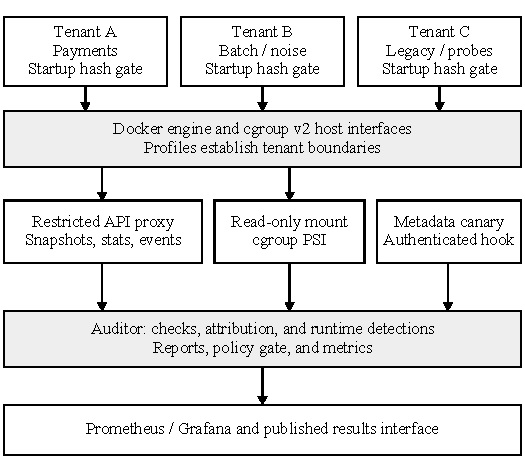
\includegraphics[width=\columnwidth]{ieee-architecture.pdf}
\caption{IsoLab observation architecture. The socket proxy carries engine observations; cgroup PSI uses a separate read-only host mount. The canary reports access through an authenticated hook. Startup gates are enabled in the revised hardened profile and postdate E1--E3 measurements.}
\label{fig:architecture}
\end{figure}

In the hardened profile, workloads run as user 10001, drop capabilities, enable no-new-privileges, and use read-only root filesystems. Process and memory limits constrain resource use. Separate internal networks and volumes establish tenant boundaries. A topology planner allocates disjoint reported physical-core groups to tenants and separate groups to the provider and load generator; CPU quotas further constrain execution. Nested virtualization means that reported core topology does not establish exclusive use of physical host cores or caches.

\begin{table}[t]
\caption{Historical R1--R4 Requirements and Implementation Evidence}
\label{tab:requirements}
\centering
\footnotesize
\renewcommand{\arraystretch}{1.14}
\begin{tabular}{@{}>{\raggedright\arraybackslash}p{.18\columnwidth}>{\raggedright\arraybackslash}p{.48\columnwidth}>{\raggedright\arraybackslash}p{.28\columnwidth}@{}}
\toprule
Req. & Mechanisms & Evidence \\ \midrule
R1 Identity & Workload and tenant labels; identity checks; canary attribution & E3 attribution \\
R2 Separation & CPU sets and quotas; network and volume boundaries; least privilege & E1 latency; E2 probes \\
R3 Observation & Five-second resource and PSI sampling; telemetry and CPU fairness rule & E1 counters; E3 noise trigger \\
R4 Examination & Engine events; privileged-start and attachment rules; metadata canary & E2 exposure; E3 triggers \\
\bottomrule
\end{tabular}
\end{table}

Docker exposes CPU quotas, CPU affinity, and memory constraints as distinct resource controls~\cite{dockerresources}. Seccomp restricts system-call access~\cite{dockerseccomp}; its configured presence reduces exposed functionality but does not prove the absence of kernel defects. Several controls change together, so the experiment estimates the effect of the configuration bundle.

\subsection{Configuration Auditing and Policy Gates}
Table~\ref{tab:requirements} maps the implementation to R1--R4. The auditor evaluates configuration checks against a snapshot and policy, groups findings by the source survey's five virtualization axes, and exports JSON and Static Analysis Results Interchange Format (SARIF) 2.1.0 reports~\cite{sarif}. Python data models generate JSON Schemas. The TypeScript interface validates published reports and independently recomputes scores. The auditor obtains engine information through a restricted socket proxy with write requests disabled; a read-only filesystem mount alone would not make an engine socket safe.

For the applicable check set $A$, coverage is
\begin{equation}
C=\frac{\sum_{i\in A} w_i c_i}{\sum_{i\in A} w_i},
\label{eq:coverage}
\end{equation}
where severity weights $w_i$ are 4, 3, 2, and 1 for critical, high, medium, and low checks. Passing checks earn credit $c_i=1$, warnings earn 0.5, and failures or errors earn 0. Waived findings also earn 0; skipped checks are excluded from $A$. This project-defined score describes posture, not compromise probability. A separate high-severity policy gate determines whether blocking findings remain.

Time-limited waivers retain provider weaknesses as visible findings. The historical hardened run waived CPU mitigation exposure (HV-03) and absence of user namespaces (HV-04). Mandatory access control (HV-05) was skipped because AppArmor or SELinux was unavailable. Waiver approval fields remain pending owner review; a computationally passing gate is therefore not evidence of documented risk acceptance.

\subsection{Runtime Observation and Detection}
Nine rules observe tenant execution, privileged starts, engine-socket mounts, host-namespace joins, missing identity, cross-tenant network attachment, canary access, excessive shared-CPU use, and out-of-memory events. Docker's event interface exposes container lifecycle and execution events~\cite{dockerevents}; IsoLab adds project-specific classification and attribution. Resource counters and PSI are sampled every five seconds. The noisy-neighbor rule identifies sustained excessive processor use on CPUs shared with another active tenant. Detection records include rule, workload, expected attribution evidence, and timestamps.

Rules describe observable behaviors rather than inferred malicious intent. Legitimate maintenance can generate similar events. Detection state is bounded and held in memory, so durable incident retention requires additional infrastructure. The experiments exercise eight trigger types; the out-of-memory rule is not included in the live detection evaluation.

\subsection{Selected ACM Defenses and Startup Integrity}
The crosswalk records six selected themes: host-mount restriction, root-filesystem immutability, least privilege, private process namespaces, syscall filtering, and resource allocation. Mount restriction implements the host-volume aspect of M1; immutability implements M3. Other associations use the survey's attack surfaces, including E18/E32, A6.1/E23, A7, and E34. These are our defensive engineering associations, not claims that a configuration check reproduces a CVE or extends the survey's own mitigation table. A theme is configuration-verified only when every mapped check and target passes without a waiver. Missing, duplicate, skipped, erroneous, or waived evidence cannot establish verification. No percentage of the complete exploit taxonomy is inferred.

For a selected aspect of M2, image builds produce SHA-256 allowlists of the interpreter, startup application, probe script, and integrity launcher; the batch image additionally includes the stress executable. SHA-256 is specified in the Secure Hash Standard~\cite{sha256}; using that hash does not authenticate the manifest or establish trusted build provenance. Hardened workloads enable a launcher that validates all recorded hashes and permits only an allowlisted executable. For Python, it additionally requires an allowlisted entry script, rejecting inline or module-mode execution through this launcher. A mismatch, missing file, unlisted command, or invalid manifest returns exit code 78 before application execution. The ordinary hardened batch job also uses this launcher. The insecure profile leaves enforcement disabled as a comparison control.

The build environment, manifest, launcher, and engine remain trusted. An engine administrator can replace the entrypoint, and an arbitrary process started through another path is not mediated. This mechanism is startup integrity checking rather than continuous attestation, complete application control, or protection against a compromised image builder. It complements the read-only filesystem instead of replacing it.

\section{Experimental Method}
\subsection{Environment and Evidence Provenance}
The historical E1--E3 measurements were generated on October 12, 2026, under source identifier \code{dffa2c70c553}. The environment records six reported physical cores, twelve logical CPUs, Docker 29.2.1, kernel 6.6.87.2-microsoft-standard-WSL2, and cgroup v2. The artifact contains protocols, per-run summaries, outcomes, and machine-readable hypotheses~\cite{artifact}. The revised defense crosswalk and E4--E5 challenges were executed on November 11, 2026. They do not update or relabel the historical latency measurements; those predate the new startup integrity mechanism.

\subsection{E1 Processor Interference}
A constant-arrival-rate k6 workload sends 50 requests per second to tenant A's \code{/work} endpoint. This open-model executor schedules iterations independently of response time while sufficient virtual users are available~\cite{k6}; dropped iterations are therefore an explicit validity condition. Each arm has 15 seconds of discarded warm-up and 90 measured seconds. Three repetitions per profile and arm produce twelve measured runs. Tenant B executes a CPU-only \code{stress-ng} job. A separate load-generator allocation limits measurement interference. The application performs 2500 SHA-256 rounds per request and reports server work time separately from request latency.

The four arms are insecure baseline, insecure noisy, hardened baseline, and hardened noisy. Arms are interleaved with cooldowns. Runs are invalid if arrival iterations are dropped, failures exceed 1\%, or the noisy job fails the protocol's processor-activity floor. The committed full run satisfies these validity conditions. The experimental SLO is a 99th-percentile request latency of at most 25~ms.

For profile $p$, the interference factor is
\begin{equation}
\mathrm{IF}_{p}=\frac{\operatorname{median}_{r} q_{.99,p,\mathrm{noisy},r}}
{\operatorname{median}_{r} q_{.99,p,\mathrm{baseline},r}},
\label{eq:if}
\end{equation}
where $q_{.99,p,a,r}$ is the request-latency quantile for repetition $r$ in arm $a$. This is a ratio of medians of run quantiles, not a quantile of pooled requests. Three run repetitions, rather than the number of requests, determine the experimental replication count.

\subsection{E2 Boundary Probes}
Twelve read-only or connection-based probes test cross-tenant DNS and IP access, a published host route, metadata and telemetry access, internet egress, process visibility, engine-socket access, host-file visibility, another tenant's nonsecret marker file, effective capabilities, and tenant-B-to-A connectivity. Three positive controls verify application health access, provider monitoring access, and local loopback connectivity. Each probe returns allowed, blocked, or error. A passing hardened result requires all twelve boundaries explicitly blocked and all three controls allowed; an error is not evidence of isolation.

\subsection{E3 Detection Validation}
Each profile first runs under normal load for 120 seconds, followed by benign triggers corresponding to unsafe execution, privilege, mounts, namespaces, missing labels, network attachment, canary access, and CPU contention. Ordinary event detections have a five-second limit, while the sustained noisy-neighbor rule has a ninety-second limit. Attribution must agree with the protocol's expected identity, which can be unknown for unlabelled workloads. Hardened trigger T7 is expected to remain silent because its dedicated CPU allocation prevents the shared-CPU detection condition. Event and observation timestamps use the same VM clock domain.

\subsection{Hypotheses and Analysis Plan}
The protocol specifies H1: insecure $\mathrm{IF}\geq2$; H2: hardened $\mathrm{IF}\leq1.25$ while meeting the latency target; optional H3: increased server time under SMT sharing; H4: noisy-neighbor detection in the insecure profile and silence in the hardened profile; H5: at least ten insecure paths open; H6: zero hardened paths open with passing controls; and H7: timely detection, expected attribution, and no observed false positives. The protocol logs detector calibration changes after smoke tests. A later evidence-validation correction strengthens acceptance predicates without changing thresholds or historical measurements.

We report run-level medians and ranges rather than statistical significance from three repetitions. For detection, illustrative Wilson intervals~\cite{wilson} show the uncertainty associated with small success counts; heterogeneous deterministic triggers do not justify treating those intervals as representative attack-detection estimates. A separately qualified Poisson calculation illustrates the limited information supplied by a short quiet window.

\subsection{E4 Configuration Faults and E5 Startup Integrity}
E4 starts with the committed hardened snapshot and independently mutates tenant A ten times: privileged execution, retained capabilities, unconfined seccomp, root execution, host PID sharing, missing CPU quota, writable root filesystem, sensitive host bind, engine-socket mount, and absent CPU placement. Each mutation starts from a fresh deep copy. Success requires the specified tenant/check pair to pass before mutation and explicitly fail afterward. Existing unrelated host failures cannot satisfy this criterion. This is a saved-snapshot checker-sensitivity experiment, not ten live attacks or ten independent deployments.

For mutation $j$, let $b_j$ and $m_j$ denote the targeted baseline and mutated check outcomes. The acceptance indicator is
\begin{equation}
d_j=\mathbf{1}\{b_j=\mathrm{pass}\ \land\ m_j=\mathrm{fail}\}.
\label{eq:fault}
\end{equation}
Only the same tenant/check pair is compared. Missing or ambiguous targets earn zero credit, and every case must satisfy the indicator for the study gate to pass. This distinguishes detection of an introduced regression from rediscovery of an existing failure.

E5 executes the actual launcher in isolated subprocesses with a temporary application that writes an execution marker. The clean case must exit successfully and create the marker; modified, missing, or unlisted scripts and an invalid manifest must return 78 without creating it. These five deliberately selected cases validate startup decisions, not general attack-detection accuracy. A separate container check exercises clean and bind-mounted altered application files in each of the three built tenant images. Neither challenge modifies a deployed tenant or a published historical result.

\section{Results and Analysis}
\subsection{Configuration Posture and Boundary Enforcement}
Table~\ref{tab:audit} summarizes the posture and segmentation results. Equation~\eqref{eq:coverage} gives 19.51\% coverage for the insecure configuration and 93.90\% for the hardened configuration, an increase of 74.39 percentage points. Twenty-nine of the thirty checks are applicable. The hardened profile has 27 passes, two waived failures, and one skip; the waived findings retain their coverage penalty.

\begin{table}[t]
\caption{Configuration and Segmentation Results}
\label{tab:audit}
\centering
\footnotesize
\renewcommand{\arraystretch}{1.15}
\begin{tabular}{@{}p{.42\columnwidth}p{.25\columnwidth}p{.27\columnwidth}@{}}
\toprule
Metric & Insecure & Hardened \\ \midrule
Weighted coverage & 16/82 (19.51\%) & 77/82 (93.90\%) \\
Passing checks & 6 & 27 \\
Failing checks & 23 & 2 (waived) \\
Skipped checks & 1 & 1 \\
High-severity gate & 15 blockers & Pass; 2 waivers \\
Open isolation paths & 12/12 & 0/12 \\
Positive controls & 3/3 & 3/3 \\
\bottomrule
\end{tabular}
\end{table}

All twelve tested isolation paths are open in the insecure profile and explicitly blocked in the hardened profile. Passing positive controls support the interpretation that hardened outcomes reflect the intended boundaries rather than complete application or network failure. They do not exclude every alternative cause of a particular connection failure or establish isolation beyond the tested endpoints and times. These results answer RQ2 for the tested path set.

\subsection{Latency Under Contention}
Table~\ref{tab:latency} and Fig.~\ref{fig:latency} show the latency results. Published interference factors are 3.799 insecure and 1.223 hardened. Recalculation using unrounded medians gives 3.7984 and 1.2225; the small discrepancy is due to the publisher dividing rounded medians. The relative noisy-arm improvement is
\begin{equation}
\Delta_{99}=100\left(1-\frac{5.6165454}{16.462774}\right)=65.88\%.
\label{eq:reduction}
\end{equation}

\begin{table}[t]
\caption{Run-Level 99th-Percentile Request Latency}
\label{tab:latency}
\centering
\footnotesize
\renewcommand{\arraystretch}{1.15}
\begin{tabular}{@{}lrr@{}}
\toprule
Profile and arm & Median (ms) & Range (ms) \\ \midrule
Insecure baseline & 4.334 & 4.320--4.492 \\
Insecure noisy & 16.463 & 16.229--16.663 \\
Hardened baseline & 4.594 & 4.535--4.628 \\
Hardened noisy & 5.617 & 5.105--5.904 \\
\bottomrule
\end{tabular}
\end{table}

\begin{figure}[t]
\centering
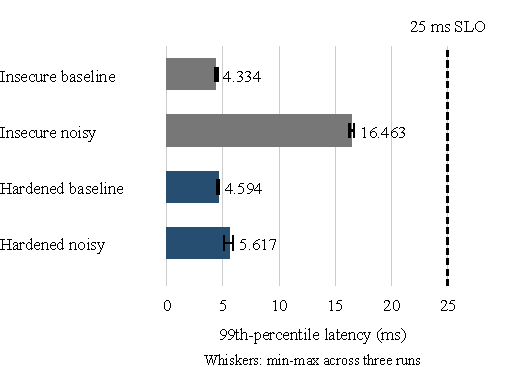
\includegraphics[width=\columnwidth]{ieee-latency.pdf}
\caption{E1 request latency. Bars show medians of run-level p99 values; whiskers show the minimum and maximum across three runs, not confidence intervals. The dashed line is the 25~ms SLO. Both profiles meet the target.}
\label{fig:latency}
\end{figure}

Hardened baseline latency is approximately 6.0\% higher than insecure baseline latency. Because the experiment changes a bundle of controls, it cannot attribute either that baseline difference or the noisy-arm reduction to a single mechanism. Both configurations remain within the 25~ms SLO, so the demonstrated benefit is reduced interference and greater latency headroom, rather than recovery from an observed SLO violation. This answers RQ1 within the tested workload.

The insecure and hardened profiles contain 27005 and 27003 measured iterations, respectively. Those requests are nested within only three repetitions per arm. With this replication count and no retained request-level traces in the published package, the observed ranges are descriptive; they do not support precise population tail estimates or a claim of statistical significance.

\subsection{Detection and Attribution}
Table~\ref{tab:detection} summarizes E3. All eight expected insecure detections and seven expected hardened detections occur within their budgets. Hardened T7 remains silent as required. The insecure maximum latency of 43.75~s belongs to the sustained CPU-contention trigger, whose budget is ninety seconds; it is not an ordinary event exceeding a five-second limit. Comparing median detection latencies between profiles as a detector-speed improvement would be confounded by their different expected trigger sets.

\begin{table}[t]
\caption{Detection Results and Expected Attribution}
\label{tab:detection}
\centering
\footnotesize
\renewcommand{\arraystretch}{1.15}
\begin{tabular}{@{}p{.49\columnwidth}rr@{}}
\toprule
Metric & Insecure & Hardened \\ \midrule
Timely expected detections & 8/8 & 7/7 \\
Expected attribution agreement & 100\% & 100\% \\
Median latency (ms) & 177.9 & 95.4 \\
Maximum latency (ms) & 43752.4 & 216.6 \\
Alerts in 120-s quiet window & 0 & 0 \\
\bottomrule
\end{tabular}
\end{table}

All fifteen expected detections match the protocol's expected attribution. This includes an unknown value for intentionally unlabelled workloads and some insecure-profile network and canary triggers. Thus 100\% agreement does not mean every event has a known tenant identity. These results answer RQ3 for the configured benign trigger set.

Illustrative Wilson 95\% intervals~\cite{wilson} for 8/8 and 7/7 successes are 67.6\%--100\% and 64.6\%--100\%. Their independent-Bernoulli assumption does not hold as a sampling model for deliberately different deterministic triggers; the intervals only contextualize the small counts. Similarly, zero alerts over two minutes does not imply a zero operational false-positive rate. Under a stationary Poisson model, the one-sided 95\% upper bound for each profile is
\begin{equation}
\lambda_{\mathrm{upper}}=\frac{-\ln(0.05)}{2}=1.50\ \mathrm{alerts/min}.
\end{equation}
Longer and more diverse benign workloads are required to estimate alert burden.

H1, H2, H4, H5, H6, and H7 meet their specified criteria. H3 is inconclusive because the optional SMT-sharing arm was not executed. This is acceptance-criterion support under the recorded conditions, not a general proof of security.

\subsection{Selected Defense Validation Results}
E4 detected all ten specified configuration faults, with a passing baseline and explicit failing tenant target in each case. Four of six mapped themes are configuration-verified for the historical hardened report; none is verified for the insecure report. The two remaining hardened themes contain provider exception targets and consequently receive no complete-verification credit under the strict all-target rule. E5 passed all five startup challenges: the clean application executed, while four invalid cases were rejected before execution. Six additional checks in real container images accepted each clean application and rejected its altered-file counterpart. These outcomes answer RQ4 for the selected inputs. They do not estimate sensitivity to unseen attacks, and configuration verification does not establish resistance to every exploit sharing the survey category.

The added contribution is the connection among a defense recommendation, its enforcement mechanism, and a reproducible counterexample test, combined with separate reliability evidence. There is no head-to-head comparison with the 2024 learned classifier and no basis for a claim of greater accuracy or comprehensive security than either source paper.

\begin{table}[t]
\caption{New Defense Validation Evidence (November 2026)}
\label{tab:newdefenses}
\centering
\footnotesize
\renewcommand{\arraystretch}{1.15}
\begin{tabular}{@{}p{.60\columnwidth}r@{}}
\toprule
Criterion & Outcome \\ \midrule
E4 specified configuration faults detected & 10/10 \\
E5 clean subprocess executed & 1/1 \\
E5 invalid subprocess inputs refused & 4/4 \\
Clean container-image checks accepted & 3/3 \\
Altered container-image checks refused & 3/3 \\
Hardened themes with all-target verification & 4/6 \\
\bottomrule
\end{tabular}
\end{table}

Table~\ref{tab:newdefenses} separates the distinct validation units. Fresh hardened smoke checks additionally preserved twelve blocked boundary paths and three allowed positive controls, detected seven expected triggers with no alerts in a thirty-second quiet window, and passed the configuration gate with the two pre-existing host waivers. This shortened smoke check does not replace the historical full-length evaluation or establish the latency performance of the revised system.

\section{Discussion and Reproducibility}
\subsection{Security and Reliability Interpretation}
The three experiments provide complementary evidence. E1 measures the reliability effect of CPU contention; E2 checks concrete exposure paths; E3 evaluates observation and attribution of selected behaviors. None can replace the others. In particular, satisfying a latency target cannot establish confidentiality, and detecting a management event cannot prove that the corresponding action was prevented. The combined results support the feasibility of integrating posture controls and SRE observations within the stated trust boundary.

Dedicated allocations also constrain resource sharing. The present study does not measure consolidation efficiency or cost, so the latency improvement should not be interpreted as a cost-free optimization. A deployment decision requires capacity and utilization measurements alongside these isolation indicators.

\subsection{Evidence Validation}
The final evidence predicates require the complete unique E2 probe set with explicit outcomes and the complete unique E3 trigger set with timely detection, expected attribution, required silence, and no false-positive records. This prevents an erroneous or missing probe from being counted as a closed path and prevents summary detection counts from hiding attribution failures. Publisher verdicts and live gates share these predicates. The stricter predicates pass the historical results.

Thirteen evidence-gate regression cases exercise valid and corrupted inputs, including missing, duplicate, late, erroneous, open, and misattributed outcomes. Additional research tests verify mutation independence, baseline contamination rejection, fail-closed mapping, references, provenance hashes, and startup challenge outcomes. The revised Python suite reports 182 passed and one skipped test; the skipped case depends on an unpublished literature extension. The frontend reports 52 passing tests. Lint and the production build pass. Software checks establish internal consistency rather than a new performance benchmark.

\subsection{Artifact Availability}
The source and machine-readable measurements are available in the project repository~\cite{artifact}. The experiment protocol records configurations, metrics, thresholds, and deviations. Full reproduction uses the lab orchestrator to check the host, execute both profiles with the full experiment variant, and publish the generated results. The reanalysis script independently recalculates scores, latency summaries, run validity, and detection outcomes, and records SHA-256 hashes of its inputs. The manuscript and IEEEtran source are supplied with the artifact.

An additional literature-replication pipeline is not a completed result of this paper. Its blind human annotation remains unfinished; development-set classifier metrics and unvalidated literature-trend hypotheses are excluded. No inference about the persistence of the 2012 literature deficit is drawn from that extension.

\section{Threats to Validity}
\subsection{Internal and Construct Validity}
The insecure baseline is deliberately weak and is not a measured average production configuration. Several controls change together, preventing causal attribution to individual settings. Monitoring overhead is unquantified because no monitoring-disabled arm was measured. Check coverage depends on project-selected severities and applicability rules; it is not a validated risk score. The detector observes behaviors that can also occur during legitimate maintenance.

The metadata canary measures access to a decoy rather than secret recovery or prevention of arbitrary exfiltration. No kernel escape, speculative-execution exploit, or cache side channel was attempted. Administrative identity labels do not supply cryptographic identity. The provider plane is trusted, and some rules observe operator-generated events that tenants cannot necessarily generate from within their confinement.

\subsection{External and Statistical Validity}
The evaluation uses one machine, a synthetic service, fixed offered load, three repetitions per arm, and short observation windows. It excludes storage and network contention, multiple hosts, scaling, sustained incidents, and workload churn. The trigger set is deterministic and too small to establish general detection sensitivity or a representative false-alarm rate. No independent baseline tool was benchmarked.

Docker Desktop's nested virtualization limits physical-core interpretation and visibility into provider mitigations. Two host findings remain waived, and mandatory access control is not evaluated on this host. The measurement source identifier predates later repository changes; fixture and schema checks do not prove that the final revision reproduces identical live measurements. Request-level load-test traces and full monitoring time series are absent from the committed published package, limiting reconstruction to supplied summaries and outcomes.

\balance
\section{Conclusion and Future Work}
IsoLab connects selected recent container-security defenses to executable checks and startup integrity enforcement, with multi-tenant reliability observation. Its new fault challenges detected ten specified configuration regressions, accepted the clean startup application, and refused four invalid startup cases. Historical single-host measurements show a 65.9\% reduction in median noisy-arm 99th-percentile latency, twelve closed exposure paths, and three preserved positive controls. Expected detection outcomes matched the protocol, and both profiles satisfied the latency target. These findings support the engineering feasibility of the selected defenses and complementary evidence under the stated trust boundary.

Future work should reproduce the final revision on multiple hosts and workloads, increase independent repetitions, retain raw traces, measure monitoring overhead, and separate the contributions of individual controls through ablation. Longer benign-operation windows, additional detection triggers, and VM-based deployments would broaden the evidence. The separate literature extension requires completed blind annotation before any trend claims are justified.

Further extensions should reproduce the 2024 learned monitoring pipeline against a deterministic baseline, quantify startup-hashing cost, add continuous file-integrity observation and signed manifests, and broaden selected ACM defense coverage. The revised system supplies executable local validation rather than evidence that the recent works are outperformed.

\begin{thebibliography}{00}
\interlinepenalty=10000
\bibitem{qos2024} P. Horchulhack, E. K. Viegas, A. O. Santin, F. V. Ramos, and P. Tedeschi, ``Detection of quality of service degradation on multi-tenant containerized services,'' \emph{Journal of Network and Computer Applications}, vol. 224, Art. no. 103839, 2024, doi: \href{https://doi.org/10.1016/j.jnca.2024.103839}{10.1016/j.jnca.2024.103839}.
\bibitem{acm2025} O. Jarkas, R. Ko, N. Dong, and R. Mahmud, ``A container security survey: Exploits, attacks, and defenses,'' \emph{ACM Computing Surveys}, vol. 57, no. 7, Art. no. 170, pp. 1--36, 2025, doi: \href{https://doi.org/10.1145/3715001}{10.1145/3715001}.
\bibitem{gonzalez} N. Gonzalez, C. Miers, F. Red\'igolo, M. Simpl\'icio, T. Carvalho, M. N\"aslund, and M. Pourzandi, ``A quantitative analysis of current security concerns and solutions for cloud computing,'' \emph{Journal of Cloud Computing}, vol. 1, Art. no. 11, 2012, doi: \href{https://doi.org/10.1186/2192-113X-1-11}{10.1186/2192-113X-1-11}.
\bibitem{sultan} S. Sultan, I. Ahmad, and T. Dimitriou, ``Container security: Issues, challenges, and the road ahead,'' \emph{IEEE Access}, vol. 7, pp. 52976--52996, 2019, doi: \href{https://doi.org/10.1109/ACCESS.2019.2911732}{10.1109/ACCESS.2019.2911732}.
\bibitem{lin2018} X. Lin, L. Lei, Y. Wang, J. Jing, K. Sun, and Q. Zhou, ``A measurement study on Linux container security: Attacks and countermeasures,'' in \emph{Proc. 34th Annual Computer Security Applications Conf.}, 2018, pp. 418--429, doi: \href{https://doi.org/10.1145/3274694.3274720}{10.1145/3274694.3274720}.
\bibitem{nist} M. Souppaya, J. Morello, and K. Scarfone, \emph{Application Container Security Guide}, NIST SP 800-190, Sep. 2017, doi: \href{https://doi.org/10.6028/NIST.SP.800-190}{10.6028/NIST.SP.800-190}.
\bibitem{felter} W. Felter, A. Ferreira, R. Rajamony, and J. Rubio, ``An updated performance comparison of virtual machines and Linux containers,'' in \emph{Proc. IEEE Int. Symp. Performance Analysis of Systems and Software}, 2015, pp. 171--172, doi: \href{https://doi.org/10.1109/ISPASS.2015.7095802}{10.1109/ISPASS.2015.7095802}.
\bibitem{cgroup} Linux Kernel Documentation, ``Control Group v2.'' Accessed: Nov. 14, 2026. [Online]. Available: \url{https://docs.kernel.org/admin-guide/cgroup-v2.html}
\bibitem{psi} Linux Kernel Documentation, ``PSI---Pressure Stall Information.'' Accessed: Nov. 14, 2026. [Online]. Available: \url{https://docs.kernel.org/accounting/psi.html}
\bibitem{sre} S. Thurgood and D. Ferguson, with A. Hidalgo and B. Beyer, ``Implementing SLOs,'' in \emph{The Site Reliability Workbook}. Sebastopol, CA, USA: O'Reilly Media, 2018. [Online]. Available: \url{https://sre.google/workbook/implementing-slos/}
\bibitem{tail} J. Dean and L. A. Barroso, ``The tail at scale,'' \emph{Communications of the ACM}, vol. 56, no. 2, pp. 74--80, 2013, doi: \href{https://doi.org/10.1145/2408776.2408794}{10.1145/2408776.2408794}.
\bibitem{scheduler} V. Varadarajan, T. Ristenpart, and M. Swift, ``Scheduler-based defenses against cross-VM side-channels,'' in \emph{Proc. 23rd USENIX Security Symp.}, 2014, pp. 687--702. [Online]. Available: \url{https://www.usenix.org/conference/usenixsecurity14/technical-sessions/presentation/varadarajan}
\bibitem{dockerresources} Docker, ``Resource constraints.'' Accessed: Nov. 14, 2026. [Online]. Available: \url{https://docs.docker.com/engine/containers/resource_constraints/}
\bibitem{dockerseccomp} Docker, ``Seccomp security profiles for Docker.'' Accessed: Nov. 14, 2026. [Online]. Available: \url{https://docs.docker.com/engine/security/seccomp/}
\bibitem{sarif} OASIS, \emph{Static Analysis Results Interchange Format (SARIF) Version 2.1.0}, OASIS Standard, Mar. 27, 2020. [Online]. Available: \url{https://docs.oasis-open.org/sarif/sarif/v2.1.0/os/sarif-v2.1.0-os.html}
\bibitem{dockerevents} Docker, ``docker system events.'' Accessed: Nov. 14, 2026. [Online]. Available: \url{https://docs.docker.com/reference/cli/docker/system/events/}
\bibitem{sha256} National Institute of Standards and Technology, \emph{Secure Hash Standard (SHS)}, FIPS PUB 180-4, Aug. 2015, doi: \href{https://doi.org/10.6028/NIST.FIPS.180-4}{10.6028/NIST.FIPS.180-4}.
\bibitem{artifact} IsoLab project, ``Cloud\_Security source, protocols, and experimental artifacts,'' measurement source dffa2c70c553, Oct. 12, 2026; integrity and fault studies Nov. 11, 2026. [Online]. Available: \url{https://github.com/alpha08-prog/Cloud_Security}
\bibitem{k6} Grafana Labs, ``Constant arrival rate,'' \emph{k6 Documentation}. Accessed: Nov. 14, 2026. [Online]. Available: \url{https://grafana.com/docs/k6/latest/using-k6/scenarios/executors/constant-arrival-rate/}
\bibitem{wilson} E. B. Wilson, ``Probable inference, the law of succession, and statistical inference,'' \emph{Journal of the American Statistical Association}, vol. 22, no. 158, pp. 209--212, 1927, doi: \href{https://doi.org/10.1080/01621459.1927.10502953}{10.1080/01621459.1927.10502953}.
\end{thebibliography}
\end{document}
